% Options for packages loaded elsewhere
\PassOptionsToPackage{unicode}{hyperref}
\PassOptionsToPackage{hyphens}{url}
%
\documentclass[
]{article}
\usepackage{lmodern}
\usepackage{amssymb,amsmath}
\usepackage{ifxetex,ifluatex}
\ifnum 0\ifxetex 1\fi\ifluatex 1\fi=0 % if pdftex
  \usepackage[T1]{fontenc}
  \usepackage[utf8]{inputenc}
  \usepackage{textcomp} % provide euro and other symbols
\else % if luatex or xetex
  \usepackage{unicode-math}
  \defaultfontfeatures{Scale=MatchLowercase}
  \defaultfontfeatures[\rmfamily]{Ligatures=TeX,Scale=1}
\fi
% Use upquote if available, for straight quotes in verbatim environments
\IfFileExists{upquote.sty}{\usepackage{upquote}}{}
\IfFileExists{microtype.sty}{% use microtype if available
  \usepackage[]{microtype}
  \UseMicrotypeSet[protrusion]{basicmath} % disable protrusion for tt fonts
}{}
\makeatletter
\@ifundefined{KOMAClassName}{% if non-KOMA class
  \IfFileExists{parskip.sty}{%
    \usepackage{parskip}
  }{% else
    \setlength{\parindent}{0pt}
    \setlength{\parskip}{6pt plus 2pt minus 1pt}}
}{% if KOMA class
  \KOMAoptions{parskip=half}}
\makeatother
\usepackage{xcolor}
\IfFileExists{xurl.sty}{\usepackage{xurl}}{} % add URL line breaks if available
\IfFileExists{bookmark.sty}{\usepackage{bookmark}}{\usepackage{hyperref}}
\hypersetup{
  pdftitle={San Fransciso Trees},
  pdfauthor={null},
  hidelinks,
  pdfcreator={LaTeX via pandoc}}
\urlstyle{same} % disable monospaced font for URLs
\usepackage[margin=1in]{geometry}
\usepackage{color}
\usepackage{fancyvrb}
\newcommand{\VerbBar}{|}
\newcommand{\VERB}{\Verb[commandchars=\\\{\}]}
\DefineVerbatimEnvironment{Highlighting}{Verbatim}{commandchars=\\\{\}}
% Add ',fontsize=\small' for more characters per line
\usepackage{framed}
\definecolor{shadecolor}{RGB}{248,248,248}
\newenvironment{Shaded}{\begin{snugshade}}{\end{snugshade}}
\newcommand{\AlertTok}[1]{\textcolor[rgb]{0.94,0.16,0.16}{#1}}
\newcommand{\AnnotationTok}[1]{\textcolor[rgb]{0.56,0.35,0.01}{\textbf{\textit{#1}}}}
\newcommand{\AttributeTok}[1]{\textcolor[rgb]{0.77,0.63,0.00}{#1}}
\newcommand{\BaseNTok}[1]{\textcolor[rgb]{0.00,0.00,0.81}{#1}}
\newcommand{\BuiltInTok}[1]{#1}
\newcommand{\CharTok}[1]{\textcolor[rgb]{0.31,0.60,0.02}{#1}}
\newcommand{\CommentTok}[1]{\textcolor[rgb]{0.56,0.35,0.01}{\textit{#1}}}
\newcommand{\CommentVarTok}[1]{\textcolor[rgb]{0.56,0.35,0.01}{\textbf{\textit{#1}}}}
\newcommand{\ConstantTok}[1]{\textcolor[rgb]{0.00,0.00,0.00}{#1}}
\newcommand{\ControlFlowTok}[1]{\textcolor[rgb]{0.13,0.29,0.53}{\textbf{#1}}}
\newcommand{\DataTypeTok}[1]{\textcolor[rgb]{0.13,0.29,0.53}{#1}}
\newcommand{\DecValTok}[1]{\textcolor[rgb]{0.00,0.00,0.81}{#1}}
\newcommand{\DocumentationTok}[1]{\textcolor[rgb]{0.56,0.35,0.01}{\textbf{\textit{#1}}}}
\newcommand{\ErrorTok}[1]{\textcolor[rgb]{0.64,0.00,0.00}{\textbf{#1}}}
\newcommand{\ExtensionTok}[1]{#1}
\newcommand{\FloatTok}[1]{\textcolor[rgb]{0.00,0.00,0.81}{#1}}
\newcommand{\FunctionTok}[1]{\textcolor[rgb]{0.00,0.00,0.00}{#1}}
\newcommand{\ImportTok}[1]{#1}
\newcommand{\InformationTok}[1]{\textcolor[rgb]{0.56,0.35,0.01}{\textbf{\textit{#1}}}}
\newcommand{\KeywordTok}[1]{\textcolor[rgb]{0.13,0.29,0.53}{\textbf{#1}}}
\newcommand{\NormalTok}[1]{#1}
\newcommand{\OperatorTok}[1]{\textcolor[rgb]{0.81,0.36,0.00}{\textbf{#1}}}
\newcommand{\OtherTok}[1]{\textcolor[rgb]{0.56,0.35,0.01}{#1}}
\newcommand{\PreprocessorTok}[1]{\textcolor[rgb]{0.56,0.35,0.01}{\textit{#1}}}
\newcommand{\RegionMarkerTok}[1]{#1}
\newcommand{\SpecialCharTok}[1]{\textcolor[rgb]{0.00,0.00,0.00}{#1}}
\newcommand{\SpecialStringTok}[1]{\textcolor[rgb]{0.31,0.60,0.02}{#1}}
\newcommand{\StringTok}[1]{\textcolor[rgb]{0.31,0.60,0.02}{#1}}
\newcommand{\VariableTok}[1]{\textcolor[rgb]{0.00,0.00,0.00}{#1}}
\newcommand{\VerbatimStringTok}[1]{\textcolor[rgb]{0.31,0.60,0.02}{#1}}
\newcommand{\WarningTok}[1]{\textcolor[rgb]{0.56,0.35,0.01}{\textbf{\textit{#1}}}}
\usepackage{graphicx,grffile}
\makeatletter
\def\maxwidth{\ifdim\Gin@nat@width>\linewidth\linewidth\else\Gin@nat@width\fi}
\def\maxheight{\ifdim\Gin@nat@height>\textheight\textheight\else\Gin@nat@height\fi}
\makeatother
% Scale images if necessary, so that they will not overflow the page
% margins by default, and it is still possible to overwrite the defaults
% using explicit options in \includegraphics[width, height, ...]{}
\setkeys{Gin}{width=\maxwidth,height=\maxheight,keepaspectratio}
% Set default figure placement to htbp
\makeatletter
\def\fps@figure{htbp}
\makeatother
\setlength{\emergencystretch}{3em} % prevent overfull lines
\providecommand{\tightlist}{%
  \setlength{\itemsep}{0pt}\setlength{\parskip}{0pt}}
\setcounter{secnumdepth}{-\maxdimen} % remove section numbering

\title{San Fransciso Trees}
\author{null}
\date{2020-12-08}

\begin{document}
\maketitle

\begin{Shaded}
\begin{Highlighting}[]
\KeywordTok{library}\NormalTok{(ggplot2)}
\KeywordTok{library}\NormalTok{(dplyr)}
\KeywordTok{library}\NormalTok{(stringr)}
\KeywordTok{library}\NormalTok{(tidyverse)}
\KeywordTok{library}\NormalTok{(here)}
\KeywordTok{library}\NormalTok{(patchwork)}
\end{Highlighting}
\end{Shaded}

Using the sf\_trees.csv dataset from Tidy Tuesday, I investigate what
the trees are like in San Francisco. The data has 192,987 observations
and 12 variables. The variables are the ID given to the tree, the legal
status of the tree, the species of the tree, the street address, the
order of the trees in the case that there are multiple trees at one
location, where the tree is on the lot, the primary caretaker of the
tree, the date it was planted, the diameter of the tree, the dimension
of the plot, the latitude the plant is at, and the longitude the tree is
planted.

\begin{Shaded}
\begin{Highlighting}[]
\NormalTok{sf <-}\StringTok{ }\KeywordTok{read.csv}\NormalTok{(}\KeywordTok{here}\NormalTok{(}\StringTok{"tidytuesday-master"}\NormalTok{, }\StringTok{"data"}\NormalTok{, }\StringTok{"2020"}\NormalTok{, }\StringTok{"2020-01-28"}\NormalTok{, }\StringTok{"sf_trees.csv"}\NormalTok{))}
\end{Highlighting}
\end{Shaded}

\hypertarget{question-1-where-are-the-trees-in-san-francisco-and-who-owns-them}{%
\section{Question 1 : Where are the trees in San Francisco and who owns
them?}\label{question-1-where-are-the-trees-in-san-francisco-and-who-owns-them}}

\begin{Shaded}
\begin{Highlighting}[]
\KeywordTok{ggplot}\NormalTok{(sf, }\KeywordTok{aes}\NormalTok{(}\DataTypeTok{x =}\NormalTok{ (longitude}\OperatorTok{*-}\DecValTok{1}\NormalTok{), }\DataTypeTok{y =}\NormalTok{ latitude, }\DataTypeTok{color =}\NormalTok{ caretaker)) }\OperatorTok{+}
\StringTok{  }\KeywordTok{geom_point}\NormalTok{(}\DataTypeTok{size =} \FloatTok{0.001}\NormalTok{, }\DataTypeTok{alpha =} \FloatTok{0.2}\NormalTok{) }\OperatorTok{+}
\StringTok{  }\KeywordTok{ylim}\NormalTok{(}\FloatTok{37.7}\NormalTok{,}\FloatTok{37.825}\NormalTok{) }\OperatorTok{+}
\StringTok{  }\KeywordTok{theme}\NormalTok{(}\DataTypeTok{legend.position =} \StringTok{"none"}\NormalTok{) }\OperatorTok{+}
\StringTok{  }\KeywordTok{scale_x_continuous}\NormalTok{(}\DataTypeTok{trans =} \StringTok{"reverse"}\NormalTok{) }\OperatorTok{+}
\StringTok{  }\KeywordTok{xlim}\NormalTok{(}\FloatTok{122.52}\NormalTok{, }\FloatTok{122.36}\NormalTok{) }\OperatorTok{+}\StringTok{   }
\StringTok{  }\KeywordTok{xlab}\NormalTok{(}\StringTok{"Longitude"}\NormalTok{) }\OperatorTok{+}
\StringTok{  }\KeywordTok{ylab}\NormalTok{(}\StringTok{"Latitude"}\NormalTok{) }\OperatorTok{+}
\StringTok{  }\KeywordTok{ggtitle}\NormalTok{(}\StringTok{"Map of the Trees in San Francisco"}\NormalTok{)}
\end{Highlighting}
\end{Shaded}

\begin{verbatim}
## Scale for 'x' is already present. Adding another scale for 'x', which will replace the existing scale.
\end{verbatim}

\begin{verbatim}
## Warning: Removed 2963 rows containing missing values (geom_point).
\end{verbatim}

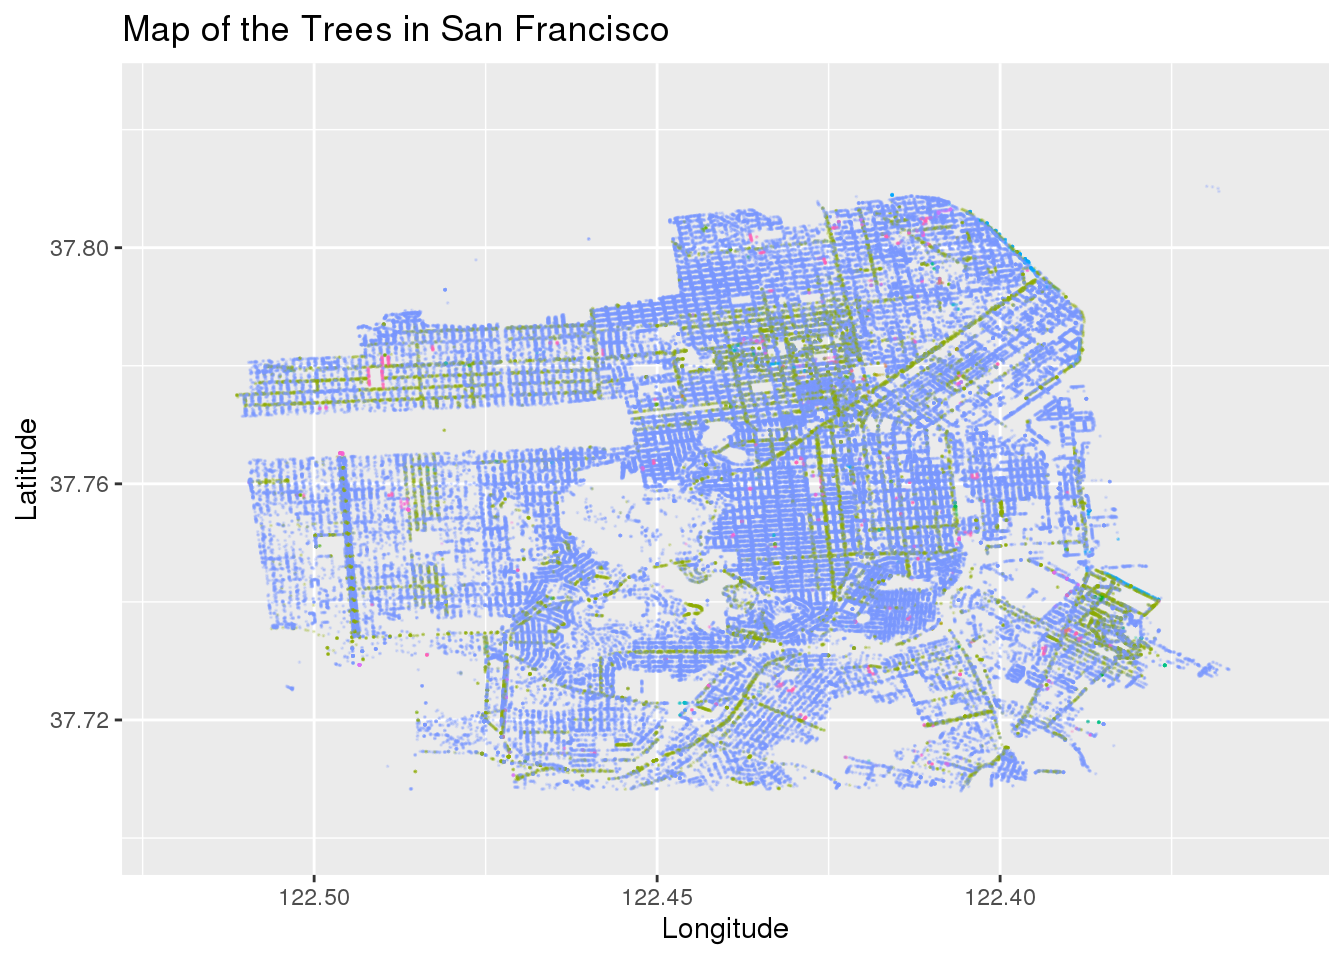
\includegraphics{index_files/figure-latex/unnamed-chunk-3-1.pdf}

This reveals that there is a lot about where the trees are in San
Francisco. A person can easily see the street layout of San Francisco.
Also, a person can see how well the streets are lined with trees. It
also shows where the data set didn't collect data, which is parks. The
long strip in the left side of the map is actually Golden Gate Park
which has several trees, but these trees were not included in the scope
of the research. The central blank area as well as the North West and
South West are areas reserved for more nature, usually golf courses. the
only area with no trees that actually has no trees is the area in the
South East. This is a primarily commercial area with few street
decorations or Trees. The blue indicates private trees, which suggests
that while the trees may be mandatory to be on a street, it is still the
land owner's responsibility to take care of the tree.

\hypertarget{question-2-what-is-the-most-common-type-of-tree}{%
\section{Question 2: What is the most common type of
tree?}\label{question-2-what-is-the-most-common-type-of-tree}}

\begin{Shaded}
\begin{Highlighting}[]
\NormalTok{species_list <-}\StringTok{ }\NormalTok{sf }\OperatorTok
\StringTok{  }\KeywordTok{mutate}\NormalTok{(}\DataTypeTok{species =} \KeywordTok{word}\NormalTok{(species, }\DecValTok{1}\NormalTok{, }\DataTypeTok{sep=}\StringTok{" "}\NormalTok{)) }\OperatorTok
\StringTok{  }\KeywordTok{separate_rows}\NormalTok{(species, }\DataTypeTok{sep =} \StringTok{' '}\NormalTok{) }\OperatorTok
\StringTok{  }\KeywordTok{group_by}\NormalTok{(species) }\OperatorTok
\StringTok{  }\KeywordTok{summarize}\NormalTok{(}\DataTypeTok{Count =} \KeywordTok{n}\NormalTok{()) }\OperatorTok
\StringTok{  }\KeywordTok{filter}\NormalTok{(Count }\OperatorTok{>=}\StringTok{ }\DecValTok{5000}\NormalTok{)}

\NormalTok{x <-}\StringTok{ }\DecValTok{0}

\ControlFlowTok{for}\NormalTok{ (i }\ControlFlowTok{in} \DecValTok{1}\OperatorTok{:}\DecValTok{12}\NormalTok{) \{}
\NormalTok{  x <-}\StringTok{ }\NormalTok{x }\OperatorTok{+}\StringTok{ }\NormalTok{species_list[i,}\DecValTok{2}\NormalTok{]}
\NormalTok{\}}

\NormalTok{z <-}\StringTok{ }\DecValTok{19287} \OperatorTok{-}\StringTok{ }\NormalTok{x}

\NormalTok{species_list[}\KeywordTok{nrow}\NormalTok{(species_list) }\OperatorTok{+}\StringTok{ }\DecValTok{1}\NormalTok{,] =}\StringTok{ }\KeywordTok{c}\NormalTok{(}\StringTok{"Other"}\NormalTok{, z)}

\KeywordTok{ggplot}\NormalTok{(species_list, }\KeywordTok{aes}\NormalTok{(}\DataTypeTok{x=} \StringTok{""}\NormalTok{, }\DataTypeTok{y=}\NormalTok{Count, }\DataTypeTok{fill =}\NormalTok{ species)) }\OperatorTok{+}
\StringTok{  }\KeywordTok{geom_bar}\NormalTok{(}\DataTypeTok{width =} \DecValTok{10}\NormalTok{, }\DataTypeTok{stat =} \StringTok{"identity"}\NormalTok{) }\OperatorTok{+}
\StringTok{  }\KeywordTok{coord_polar}\NormalTok{(}\StringTok{"y"}\NormalTok{, }\DataTypeTok{start =} \DecValTok{0}\NormalTok{) }\OperatorTok{+}
\StringTok{  }\KeywordTok{xlab}\NormalTok{(}\StringTok{" "}\NormalTok{) }\OperatorTok{+}
\StringTok{  }\KeywordTok{ylab}\NormalTok{(}\StringTok{" "}\NormalTok{) }\OperatorTok{+}
\StringTok{  }\KeywordTok{ggtitle}\NormalTok{(}\StringTok{"Number of Trees of a Certain Species"}\NormalTok{)}
\end{Highlighting}
\end{Shaded}

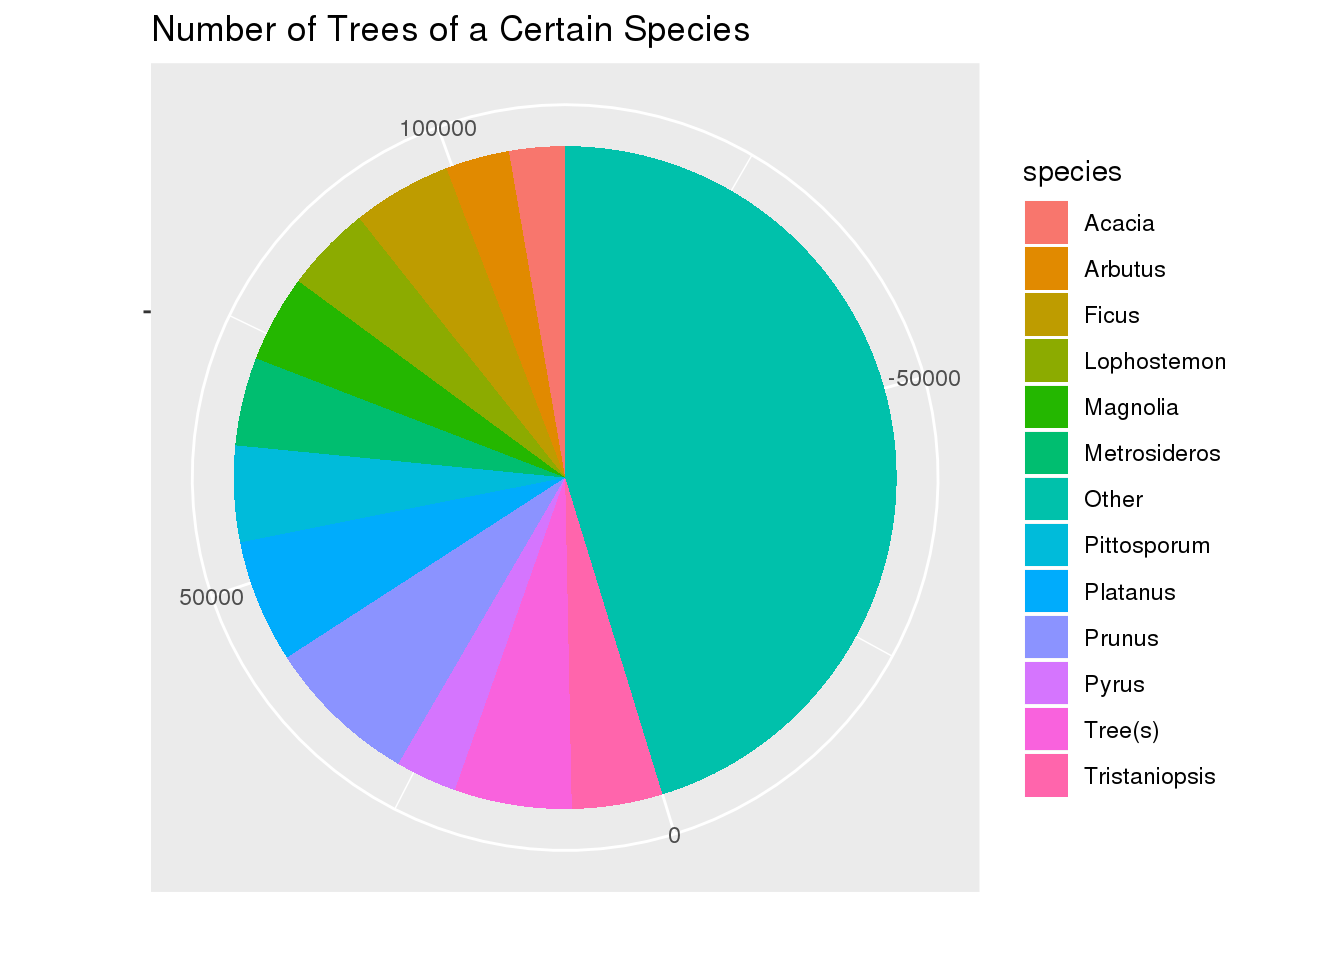
\includegraphics{index_files/figure-latex/unnamed-chunk-4-1.pdf}

Surprisingly, there is a lot of variety in tree. About 50\% of trees
have less than 5000 of the same type of tree. Considering there are
around 200,000 trees, it means that only 11 tree types are over 2.5\% of
the trees in the San Francisco area. This indicates that the people care
about their yards and their plants and want their yards to be more
unique and have personality, so they choose a more unique tree. The area
also must be habitable for any different tree types because there is so
much of a variety. If there was a large potion of any one type of tree,
it would be assumed that there is a smaller tree pool to choose from for
consumers. However, it looks like people have found that many trees can
grow well in the San Francisco area.

\hypertarget{question-3-does-site-of-the-tree-affect-the-diameter-of-the-tree}{%
\section{Question 3: Does site of the tree affect the diameter of the
tree?}\label{question-3-does-site-of-the-tree-affect-the-diameter-of-the-tree}}

\begin{Shaded}
\begin{Highlighting}[]
\NormalTok{g1 <-}\StringTok{ }\KeywordTok{ggplot}\NormalTok{(sf, }\KeywordTok{aes}\NormalTok{(}\DataTypeTok{x=}\NormalTok{ site_info)) }\OperatorTok{+}
\StringTok{  }\KeywordTok{geom_bar}\NormalTok{() }\OperatorTok{+}
\StringTok{  }\KeywordTok{theme}\NormalTok{(}\DataTypeTok{axis.text.x =} \KeywordTok{element_text}\NormalTok{(}\DataTypeTok{angle =} \DecValTok{90}\NormalTok{)) }\OperatorTok{+}
\StringTok{  }\KeywordTok{xlab}\NormalTok{(}\StringTok{"Tree Location"}\NormalTok{) }\OperatorTok{+}
\StringTok{  }\KeywordTok{ylab}\NormalTok{(}\StringTok{"Number of Trees"}\NormalTok{) }\OperatorTok{+}
\StringTok{  }\KeywordTok{ggtitle}\NormalTok{(}\StringTok{"Popular Locations of Trees in SF"}\NormalTok{)}

\NormalTok{g2 <-}\StringTok{ }\KeywordTok{ggplot}\NormalTok{(sf, }\KeywordTok{aes}\NormalTok{(}\DataTypeTok{x=}\NormalTok{ site_info)) }\OperatorTok{+}
\StringTok{  }\KeywordTok{geom_bar}\NormalTok{() }\OperatorTok{+}
\StringTok{  }\KeywordTok{theme}\NormalTok{(}\DataTypeTok{axis.text.x =} \KeywordTok{element_text}\NormalTok{(}\DataTypeTok{angle =} \DecValTok{90}\NormalTok{)) }\OperatorTok{+}\StringTok{ }
\StringTok{  }\KeywordTok{ylim}\NormalTok{(}\DecValTok{0}\NormalTok{,}\DecValTok{12500}\NormalTok{) }\OperatorTok{+}
\StringTok{  }\KeywordTok{xlab}\NormalTok{(}\StringTok{"Tree Location"}\NormalTok{) }\OperatorTok{+}
\StringTok{  }\KeywordTok{ylab}\NormalTok{(}\StringTok{"Number of Trees"}\NormalTok{) }\OperatorTok{+}
\StringTok{  }\KeywordTok{ggtitle}\NormalTok{(}\StringTok{"Locations Excluding Curbside Cutouts"}\NormalTok{)}

\NormalTok{g1 }\OperatorTok{+}\StringTok{ }\NormalTok{g2}
\end{Highlighting}
\end{Shaded}

\begin{verbatim}
## Warning: Removed 1 rows containing missing values (geom_bar).
\end{verbatim}

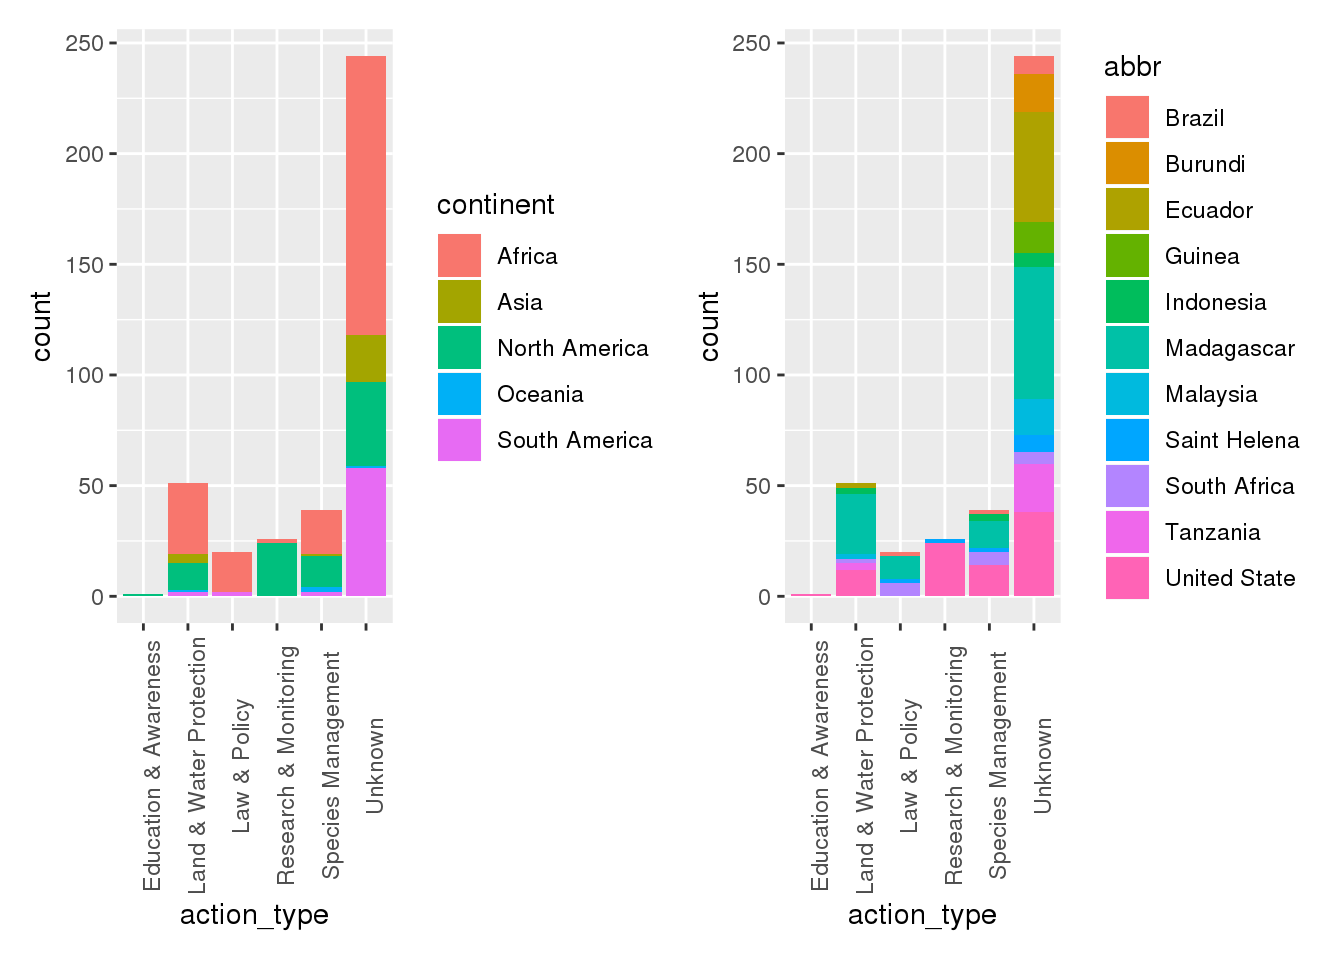
\includegraphics{index_files/figure-latex/unnamed-chunk-5-1.pdf}

As seen in the graph, a majority of the trees are on sidewalk curbs.
This is most likely why we see such a distinct street layout in the
spatial map. These trees most likely consists of the more common tree
types because they are on streets. Since they are on streets, it
suggests that there is some degree of uniformity set in place by some
form of city official or home owners association. Of the relatively
smaller tree locations, they are mostly in yards. This I believe is
where the variation in tree types comes from. In yards, it is more
likely that people can take more creative freedom on what kind of tree
they want. While some trees look nice on a curb, other more exciting and
unique trees are in private yards to add more character to one's home.

\begin{Shaded}
\begin{Highlighting}[]
\NormalTok{today <-}\StringTok{ }\DecValTok{2020}

\NormalTok{tree_age <-}\StringTok{ }\NormalTok{sf }\OperatorTok
\StringTok{  }\KeywordTok{filter}\NormalTok{(}\OperatorTok{!}\KeywordTok{is.na}\NormalTok{(dbh)) }\OperatorTok
\StringTok{  }\KeywordTok{mutate}\NormalTok{(}\DataTypeTok{age =} \KeywordTok{substr}\NormalTok{(date, }\DecValTok{1}\NormalTok{,}\DecValTok{4}\NormalTok{)) }\OperatorTok
\StringTok{  }\KeywordTok{mutate}\NormalTok{(}\DataTypeTok{age =} \KeywordTok{as.numeric}\NormalTok{(age)) }\OperatorTok
\StringTok{  }\KeywordTok{mutate}\NormalTok{(}\DataTypeTok{age =}\NormalTok{ today }\OperatorTok{-}\StringTok{ }\NormalTok{age)}
  
\NormalTok{tree_age}
\end{Highlighting}
\end{Shaded}

\begin{verbatim}
##    tree_id   legal_status                                                                   species            address site_order                    site_info caretaker       date
## 1    30314 DPW Maintained                                    Pittosporum undulatum :: Victorian Box    501 Arkansas St          1 Sidewalk: Curb side : Cutout   Private 1955-10-20
## 2    30321 DPW Maintained                                 Magnolia grandiflora :: Southern Magnolia 2828 Divisadero St          1 Sidewalk: Curb side : Cutout   Private 1956-01-06
## 3    30334 DPW Maintained                                          Ginkgo biloba :: Maidenhair Tree        601 29th St          2 Sidewalk: Curb side : Cutout   Private 1956-02-06
## 4    30335 DPW Maintained                                          Ginkgo biloba :: Maidenhair Tree        601 29th St          3 Sidewalk: Curb side : Cutout   Private 1956-02-06
## 5    30333 DPW Maintained                                Arbutus 'Marina' :: Hybrid Strawberry Tree        601 29th St          1 Sidewalk: Curb side : Cutout   Private 1956-02-06
## 6    30339 DPW Maintained                            Platanus x hispanica :: Sycamore: London Plane 2560 Divisadero St          2 Sidewalk: Curb side : Cutout   Private 1956-02-15
## 7    30337 DPW Maintained                            Platanus x hispanica :: Sycamore: London Plane 2560 Divisadero St          3 Sidewalk: Curb side : Cutout   Private 1956-02-15
## 8    30341 DPW Maintained                                    Acacia melanoxylon :: Blackwood Acacia   3789 Fillmore St          1 Sidewalk: Curb side : Cutout   Private 1956-02-15
## 9    30348 DPW Maintained                                           Ulmus parvifolia :: Chinese Elm    420 Arkansas St          1 Sidewalk: Curb side : Cutout   Private 1956-02-16
## 10   30350 DPW Maintained                                               Persea americana :: Avocado    440 Arkansas St          1 Sidewalk: Curb side : Cutout   Private 1956-02-16
## 11   53216 DPW Maintained                                     Cercis occidentalis :: Western Redbud    828 Arkansas St          1 Sidewalk: Curb side : Cutout   Private 1956-02-16
## 12   30353 DPW Maintained                                    Pittosporum undulatum :: Victorian Box    565 Arkansas St          1 Sidewalk: Curb side : Cutout   Private 1956-02-16
## 13   30346 DPW Maintained                                    Pittosporum undulatum :: Victorian Box    410 Arkansas St          1 Sidewalk: Curb side : Cutout   Private 1956-02-16
## 14   30352 DPW Maintained                                    Pittosporum undulatum :: Victorian Box    529 Arkansas St          1 Sidewalk: Curb side : Cutout   Private 1956-02-16
## 15   30351 DPW Maintained                                    Pittosporum undulatum :: Victorian Box    446 Arkansas St          1 Sidewalk: Curb side : Cutout   Private 1956-02-16
## 16   30379 DPW Maintained                                                 Maytenus boaria :: Mayten    826 Arkansas St          1 Sidewalk: Curb side : Cutout   Private 1956-03-02
## 17   30372 DPW Maintained                                           Ulmus parvifolia :: Chinese Elm   498x Arkansas St          1 Sidewalk: Curb side : Cutout   Private 1956-03-02
## 18   30362 DPW Maintained                                    Pittosporum undulatum :: Victorian Box    606 Arkansas St          1 Sidewalk: Curb side : Cutout   Private 1956-03-02
## 19   30367 DPW Maintained                                    Pittosporum undulatum :: Victorian Box    674 Arkansas St          1 Sidewalk: Curb side : Cutout   Private 1956-03-03
## 20   30368 DPW Maintained                               Fraxinus uhdei :: Shamel Ash: Evergreen Ash    406 Arkansas St          1 Sidewalk: Curb side : Cutout   Private 1956-03-03
## 21   30418 DPW Maintained                            Platanus x hispanica :: Sycamore: London Plane    2509 Filbert St          1 Sidewalk: Curb side : Cutout   Private 1956-03-26
## 22   30417 DPW Maintained Ficus microcarpa nitida 'Green Gem' :: Indian Laurel Fig Tree 'Green Gem'    2540 Filbert St          3 Sidewalk: Curb side : Cutout   Private 1956-03-26
## 23   30416 DPW Maintained Ficus microcarpa nitida 'Green Gem' :: Indian Laurel Fig Tree 'Green Gem'    2540 Filbert St          2 Sidewalk: Curb side : Cutout   Private 1956-03-26
## 24   30414 DPW Maintained                            Platanus x hispanica :: Sycamore: London Plane    2533 Filbert St          1 Sidewalk: Curb side : Cutout   Private 1956-03-26
## 25   30415 DPW Maintained Ficus microcarpa nitida 'Green Gem' :: Indian Laurel Fig Tree 'Green Gem'    2540 Filbert St          1 Sidewalk: Curb side : Cutout   Private 1956-03-26
## 26   30411 DPW Maintained                            Platanus x hispanica :: Sycamore: London Plane    2515 Filbert St          2 Sidewalk: Curb side : Cutout   Private 1956-03-27
## 27   30410 DPW Maintained                            Platanus x hispanica :: Sycamore: London Plane    2515 Filbert St          1 Sidewalk: Curb side : Cutout   Private 1956-03-27
## 28   30450 DPW Maintained                            Platanus x hispanica :: Sycamore: London Plane   3030 Pacific Ave          1 Sidewalk: Curb side : Cutout   Private 1956-05-11
## 29   30437 DPW Maintained                                                     Tristania conferta ::       567 Union St          1 Sidewalk: Curb side : Cutout   Private 1956-05-11
## 30   30431 DPW Maintained                                    Pittosporum undulatum :: Victorian Box    255 Chestnut St          1 Sidewalk: Curb side : Cutout   Private 1956-05-11
## 31   30429 DPW Maintained                                       Cinnamomum camphora :: Camphor Tree       418 Union St          1 Sidewalk: Curb side : Cutout   Private 1956-05-11
## 32   30460 DPW Maintained                                    Pittosporum undulatum :: Victorian Box       470 Union St          1 Sidewalk: Curb side : Cutout   Private 1956-05-11
## 33   30445 DPW Maintained Ficus microcarpa nitida 'Green Gem' :: Indian Laurel Fig Tree 'Green Gem'       350 Union St          3 Sidewalk: Curb side : Cutout   Private 1956-05-11
## 34   30459 DPW Maintained                            Platanus x hispanica :: Sycamore: London Plane       325 Union St          1 Sidewalk: Curb side : Cutout   Private 1956-05-11
## 35   30457 DPW Maintained                            Platanus x hispanica :: Sycamore: London Plane       331 Union St          1 Sidewalk: Curb side : Cutout   Private 1956-05-11
## 36   30454 DPW Maintained                                    Pittosporum undulatum :: Victorian Box       381 Union St          1 Sidewalk: Curb side : Cutout   Private 1956-05-11
## 37   30463 DPW Maintained                                    Pittosporum undulatum :: Victorian Box       453 Union St          1 Sidewalk: Curb side : Cutout   Private 1956-05-11
## 38   30446 DPW Maintained                                    Pittosporum undulatum :: Victorian Box       357 Union St          1 Sidewalk: Curb side : Cutout   Private 1956-05-11
## 39   30442 DPW Maintained Ficus microcarpa nitida 'Green Gem' :: Indian Laurel Fig Tree 'Green Gem'       350 Union St          4 Sidewalk: Curb side : Cutout   Private 1956-05-11
## 40   30433 DPW Maintained                            Platanus x hispanica :: Sycamore: London Plane       341 Union St          1 Sidewalk: Curb side : Cutout   Private 1956-05-11
## 41   30465 DPW Maintained                                    Pittosporum undulatum :: Victorian Box    263 Chestnut St          2 Sidewalk: Curb side : Cutout   Private 1956-05-11
## 42   30428 DPW Maintained                                    Pittosporum undulatum :: Victorian Box       434 Union St          1 Sidewalk: Curb side : Cutout   Private 1956-05-11
## 43   30451 DPW Maintained                                    Pittosporum undulatum :: Victorian Box    298 Chestnut St          1 Sidewalk: Curb side : Cutout   Private 1956-05-11
## 44   30443 DPW Maintained Ficus microcarpa nitida 'Green Gem' :: Indian Laurel Fig Tree 'Green Gem'       350 Union St          2 Sidewalk: Curb side : Cutout   Private 1956-05-11
## 45   30441 DPW Maintained Ficus microcarpa nitida 'Green Gem' :: Indian Laurel Fig Tree 'Green Gem'       350 Union St          5 Sidewalk: Curb side : Cutout   Private 1956-05-11
## 46   30440 DPW Maintained                            Platanus x hispanica :: Sycamore: London Plane       364 Union St          1 Sidewalk: Curb side : Cutout   Private 1956-05-11
## 47   30425 DPW Maintained                                Arbutus 'Marina' :: Hybrid Strawberry Tree       367 Union St          1 Sidewalk: Curb side : Cutout   Private 1956-05-11
## 48   30452 DPW Maintained                                    Pittosporum undulatum :: Victorian Box    273 Chestnut St          1 Sidewalk: Curb side : Cutout   Private 1956-05-11
## 49   30434 DPW Maintained                                    Pittosporum undulatum :: Victorian Box       312 Union St          1 Sidewalk: Curb side : Cutout   Private 1956-05-11
## 50   30438 DPW Maintained                                    Pittosporum undulatum :: Victorian Box       324 Union St          1 Sidewalk: Curb side : Cutout   Private 1956-05-11
## 51   30466 DPW Maintained                                    Pittosporum undulatum :: Victorian Box    263 Chestnut St          1 Sidewalk: Curb side : Cutout   Private 1956-05-11
## 52   30464 DPW Maintained                                    Pittosporum undulatum :: Victorian Box       460 Union St          1 Sidewalk: Curb side : Cutout   Private 1956-05-11
## 53   30444 DPW Maintained Ficus microcarpa nitida 'Green Gem' :: Indian Laurel Fig Tree 'Green Gem'       350 Union St          1 Sidewalk: Curb side : Cutout   Private 1956-05-11
## 54   30458 DPW Maintained                                Arbutus 'Marina' :: Hybrid Strawberry Tree       319 Union St          1 Sidewalk: Curb side : Cutout   Private 1956-05-11
## 55   30439 DPW Maintained                                    Pittosporum undulatum :: Victorian Box       387 Union St          1 Sidewalk: Curb side : Cutout   Private 1956-05-11
## 56   30468 DPW Maintained                                        Melaleuca quinquenervia :: Cajeput       485 Union St          2 Sidewalk: Curb side : Cutout   Private 1956-05-29
## 57   30462 DPW Maintained                                    Pittosporum undulatum :: Victorian Box       440 Union St          1 Sidewalk: Curb side : Cutout   Private 1956-05-29
## 58   30470 DPW Maintained                                        Melaleuca quinquenervia :: Cajeput       485 Union St          3 Sidewalk: Curb side : Cutout   Private 1956-05-29
## 59   30473 DPW Maintained                                    Pittosporum undulatum :: Victorian Box    274 Chestnut St          1 Sidewalk: Curb side : Cutout   Private 1956-05-29
## 60   30475 DPW Maintained                                 Callistemon citrinus :: Lemon Bottlebrush       424 Union St          1 Sidewalk: Curb side : Cutout   Private 1956-06-14
## 61   30477 DPW Maintained                             Metrosideros excelsa :: New Zealand Xmas Tree      2424 Green St          2 Sidewalk: Curb side : Cutout   Private 1956-06-14
## 62   30474 DPW Maintained                                    Pittosporum undulatum :: Victorian Box       401 Union St          1 Sidewalk: Curb side : Cutout   Private 1956-06-14
## 63   30478 DPW Maintained                                               Olea europaea :: Olive Tree      2424 Green St          3 Sidewalk: Curb side : Cutout   Private 1956-06-14
## 64   30479 DPW Maintained                             Metrosideros excelsa :: New Zealand Xmas Tree      2424 Green St          1 Sidewalk: Curb side : Cutout   Private 1956-06-14
## 65   30285 DPW Maintained                                           Ulmus parvifolia :: Chinese Elm     1355 Taylor St          1 Sidewalk: Curb side : Cutout   Private 1956-07-06
## 66   30286 DPW Maintained                                           Ulmus parvifolia :: Chinese Elm     1355 Taylor St          2 Sidewalk: Curb side : Cutout   Private 1956-07-06
## 67   30288 DPW Maintained                                           Ulmus parvifolia :: Chinese Elm     1365 Taylor St          1 Sidewalk: Curb side : Cutout   Private 1956-07-06
## 68   30298 DPW Maintained                                    Pittosporum undulatum :: Victorian Box   2751 Buchanan St          1 Sidewalk: Curb side : Cutout   Private 1956-07-24
## 69   30295 DPW Maintained                                                 Maytenus boaria :: Mayten   2752 Buchanan St          1 Sidewalk: Curb side : Cutout   Private 1956-07-24
## 70   30297 DPW Maintained                                    Acacia melanoxylon :: Blackwood Acacia   2734 Buchanan St          1 Sidewalk: Curb side : Cutout   Private 1956-07-24
## 71   30292 DPW Maintained Ficus microcarpa nitida 'Green Gem' :: Indian Laurel Fig Tree 'Green Gem'   2741 Buchanan St          1 Sidewalk: Curb side : Cutout   Private 1956-07-24
## 72   30302 DPW Maintained                                    Acacia melanoxylon :: Blackwood Acacia   2742 Buchanan St          1 Sidewalk: Curb side : Cutout   Private 1956-07-24
## 73   30299 DPW Maintained Ficus microcarpa nitida 'Green Gem' :: Indian Laurel Fig Tree 'Green Gem'   2746 Buchanan St          1 Sidewalk: Curb side : Cutout   Private 1956-07-24
## 74   30489 DPW Maintained Ficus microcarpa nitida 'Green Gem' :: Indian Laurel Fig Tree 'Green Gem'        947 Bush St          3 Sidewalk: Curb side : Cutout   Private 1956-09-05
## 75   30488 DPW Maintained Ficus microcarpa nitida 'Green Gem' :: Indian Laurel Fig Tree 'Green Gem'        947 Bush St          2 Sidewalk: Curb side : Cutout   Private 1956-09-05
## 76   30490 DPW Maintained Ficus microcarpa nitida 'Green Gem' :: Indian Laurel Fig Tree 'Green Gem'        947 Bush St          4 Sidewalk: Curb side : Cutout   Private 1956-09-05
##    dbh plot_size latitude longitude age
## 1   16      <NA> 37.75977 -122.3981  65
## 2    2      <NA> 37.79572 -122.4419  64
## 3    4      <NA> 37.74322 -122.4336  64
## 4    2      <NA> 37.74323 -122.4336  64
## 5    1      <NA> 37.74322 -122.4337  64
## 6   11      <NA> 37.79319 -122.4414  64
## 7   12      <NA> 37.79324 -122.4414  64
## 8   10      <NA> 37.80591 -122.4375  64
## 9   13      <NA> 37.76083 -122.3984  64
## 10  20      <NA> 37.76065 -122.3984  64
## 11   1      <NA> 37.75568 -122.3979  64
## 12  20      <NA> 37.75901 -122.3980  64
## 13  30      <NA> 37.76090 -122.3984  64
## 14  21      <NA> 37.75947 -122.3981  64
## 15  13      <NA> 37.76043 -122.3984  64
## 16   9      <NA> 37.75572 -122.3979  64
## 17  10       3x3 37.76005 -122.3983  64
## 18  11      <NA> 37.75852 -122.3982  64
## 19  23      <NA> 37.75779 -122.3981  64
## 20  43      <NA> 37.76105 -122.3985  64
## 21  12      <NA> 37.79730 -122.4409  64
## 22  13      <NA> 37.79741 -122.4412  64
## 23  14      <NA> 37.79742 -122.4411  64
## 24   9      <NA> 37.79725 -122.4412  64
## 25  13      <NA> 37.79739 -122.4411  64
## 26  12      <NA> 37.79729 -122.4409  64
## 27  12      <NA> 37.79728 -122.4410  64
## 28   9      <NA> 37.79209 -122.4452  64
## 29  12      <NA> 37.80044 -122.4087  64
## 30   9      <NA> 37.80438 -122.4076  64
## 31  19      <NA> 37.80085 -122.4064  64
## 32  19       4x4 37.80074 -122.4073  64
## 33  15      <NA> 37.80102 -122.4051  64
## 34   7      <NA> 37.80091 -122.4049  64
## 35   7      <NA> 37.80090 -122.4049  64
## 36   8       3x3 37.80081 -122.4057  64
## 37  16      <NA> 37.80066 -122.4069  64
## 38  12      <NA> 37.80084 -122.4054  64
## 39  14      <NA> 37.80101 -122.4051  64
## 40   8      <NA> 37.80089 -122.4051  64
## 41   7      <NA> 37.80438 -122.4077  64
## 42  13       7x3 37.80082 -122.4066  64
## 43  11      <NA> 37.80446 -122.4081  64
## 44  15      <NA> 37.80102 -122.4051  64
## 45  12      <NA> 37.80100 -122.4052  64
## 46  11      <NA> 37.80097 -122.4055  64
## 47   5      <NA> 37.80083 -122.4055  64
## 48  11      <NA> 37.80436 -122.4078  64
## 49  20      <NA> 37.80105 -122.4048  64
## 50  15      <NA> 37.80104 -122.4049  64
## 51  11      <NA> 37.80437 -122.4077  64
## 52  11      <NA> 37.80077 -122.4071  64
## 53  10      <NA> 37.80102 -122.4050  64
## 54   8      <NA> 37.80092 -122.4048  64
## 55  15      <NA> 37.80080 -122.4058  64
## 56   8       3x3 37.80061 -122.4073  64
## 57  12      <NA> 37.80081 -122.4067  64
## 58   8       3x3 37.80062 -122.4073  64
## 59  15      <NA> 37.80448 -122.4080  64
## 60   8      <NA> 37.80083 -122.4065  64
## 61  12      <NA> 37.79573 -122.4391  64
## 62   9      <NA> 37.80075 -122.4062  64
## 63   4      <NA> 37.79576 -122.4391  64
## 64  10      <NA> 37.79575 -122.4390  64
## 65   8      <NA> 37.79501 -122.4132  64
## 66  10      <NA> 37.79495 -122.4132  64
## 67  14      <NA> 37.79509 -122.4132  64
## 68  10      <NA> 37.79533 -122.4318  64
## 69  11      <NA> 37.79541 -122.4317  64
## 70   9      <NA> 37.79521 -122.4316  64
## 71  12      <NA> 37.79526 -122.4318  64
## 72  11      <NA> 37.79528 -122.4317  64
## 73  15      <NA> 37.79535 -122.4317  64
## 74  16      <NA> 37.78958 -122.4127  64
## 75  14      <NA> 37.78957 -122.4128  64
## 76  16       3x3 37.78959 -122.4127  64
##  [ reached 'max' / getOption("max.print") -- omitted 151092 rows ]
\end{verbatim}

\begin{Shaded}
\begin{Highlighting}[]
\NormalTok{b1 <-}\StringTok{ }\KeywordTok{ggplot}\NormalTok{(tree_age, }\KeywordTok{aes}\NormalTok{(}\DataTypeTok{x=}\NormalTok{ site_info, }\DataTypeTok{y =}\NormalTok{ dbh)) }\OperatorTok{+}
\StringTok{  }\KeywordTok{geom_boxplot}\NormalTok{() }\OperatorTok{+}
\StringTok{  }\KeywordTok{theme}\NormalTok{(}\DataTypeTok{axis.text.x =} \KeywordTok{element_text}\NormalTok{(}\DataTypeTok{angle =} \DecValTok{90}\NormalTok{)) }\OperatorTok{+}
\StringTok{  }\KeywordTok{ylim}\NormalTok{(}\DecValTok{0}\NormalTok{,}\DecValTok{125}\NormalTok{) }\OperatorTok{+}
\StringTok{  }\KeywordTok{xlab}\NormalTok{(}\StringTok{"Tree Location"}\NormalTok{) }\OperatorTok{+}
\StringTok{  }\KeywordTok{ylab}\NormalTok{(}\StringTok{"Diameter"}\NormalTok{) }\OperatorTok{+}
\StringTok{  }\KeywordTok{ggtitle}\NormalTok{(}\StringTok{"Diameter of Tree per Location"}\NormalTok{)}

\NormalTok{b2 <-}\StringTok{ }\KeywordTok{ggplot}\NormalTok{(tree_age, }\KeywordTok{aes}\NormalTok{(}\DataTypeTok{x=}\NormalTok{ site_info, }\DataTypeTok{y =}\NormalTok{ age)) }\OperatorTok{+}
\StringTok{  }\KeywordTok{geom_boxplot}\NormalTok{() }\OperatorTok{+}
\StringTok{  }\KeywordTok{theme}\NormalTok{(}\DataTypeTok{axis.text.x =} \KeywordTok{element_text}\NormalTok{(}\DataTypeTok{angle =} \DecValTok{90}\NormalTok{)) }\OperatorTok{+}
\StringTok{  }\KeywordTok{ylim}\NormalTok{(}\DecValTok{0}\NormalTok{,}\DecValTok{70}\NormalTok{) }\OperatorTok{+}
\StringTok{  }\KeywordTok{xlab}\NormalTok{(}\StringTok{"Tree Location"}\NormalTok{) }\OperatorTok{+}
\StringTok{  }\KeywordTok{ylab}\NormalTok{(}\StringTok{"Age"}\NormalTok{) }\OperatorTok{+}
\StringTok{  }\KeywordTok{ggtitle}\NormalTok{(}\StringTok{"Age of Tree per Location"}\NormalTok{)}

\NormalTok{b1 }\OperatorTok{+}\StringTok{ }\NormalTok{b2}
\end{Highlighting}
\end{Shaded}

\begin{verbatim}
## Warning: Removed 13 rows containing non-finite values (stat_boxplot).
\end{verbatim}

\begin{verbatim}
## Warning: Removed 113239 rows containing non-finite values (stat_boxplot).
\end{verbatim}

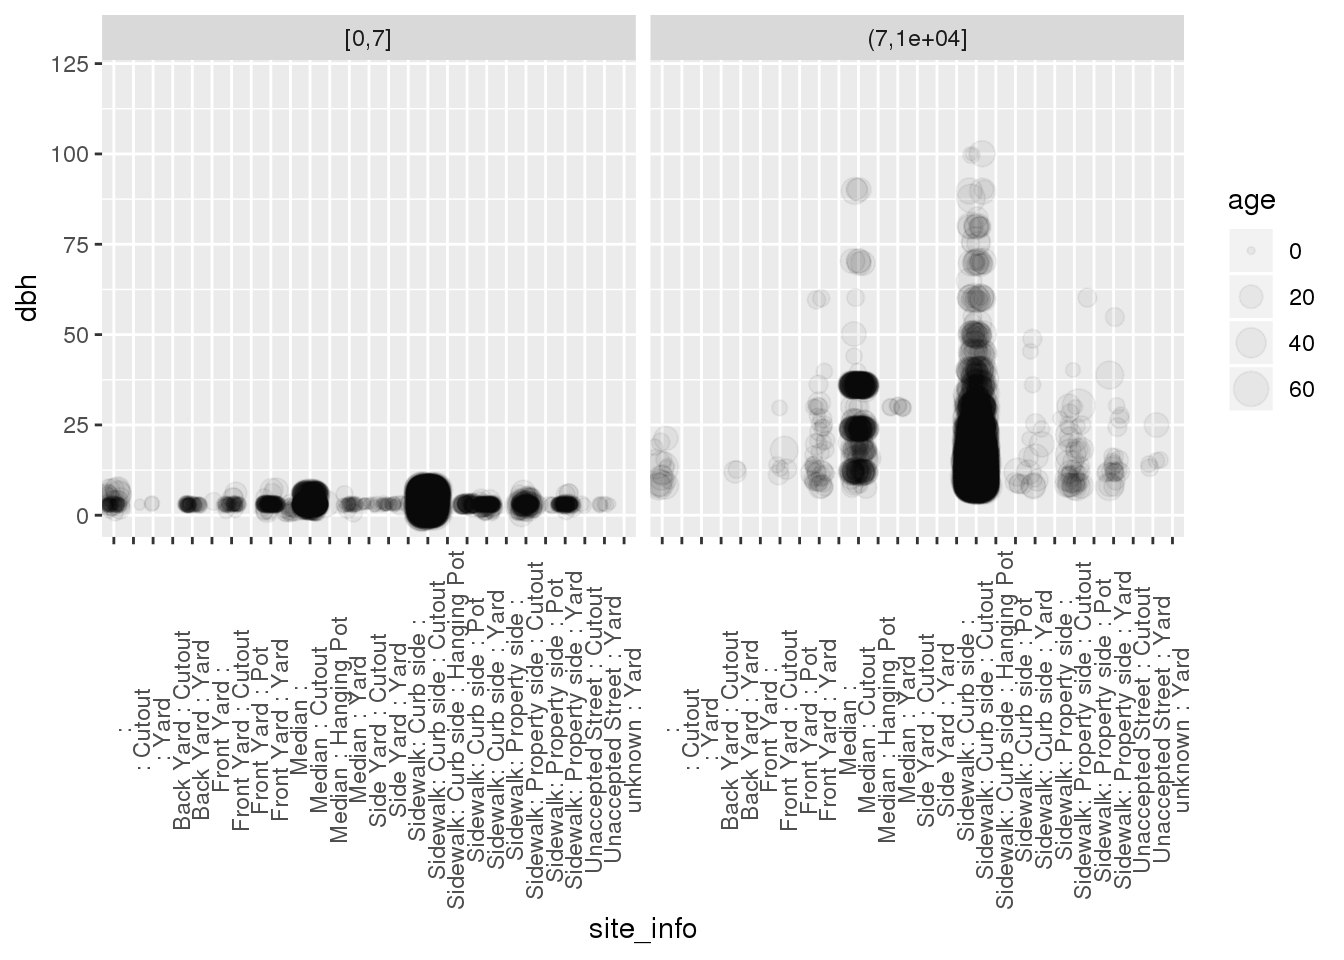
\includegraphics{index_files/figure-latex/unnamed-chunk-6-1.pdf}

These graphs shows that trees that grow in yards grow bigger for their
age then other trees. While other spots may use trees as decoration,
trees should be in the place where they grow the best.

\hypertarget{conclusion}{%
\section{Conclusion}\label{conclusion}}

San Francisco has many beautiful trees in its cities that like to line
the roads and street layout. It also has many trees that are in large
parks as well as in people's personal yards. There is a lot of variation
in the tree types, and no one tree has near a large portion at all. This
adds to the diversity of the city However, if trees grew in yards, the
trees would grow bigger and better.

\end{document}
